\chapter{绪论}

% --- 兼容性宏：若主文档未加载 amsmath/amsfonts，可避免 \eqref/\mathbb 报错 ---
\providecommand{\eqref}[1]{(\ref{#1})}
\providecommand{\mathbb}[1]{\mathbf{#1}}
% ------------------------------------------------------------------------

随着计算机图形学的发展，其研究目标已由早期面向光栅显示和离线渲染的图像合成，逐步扩展为涵盖几何建模、物理仿真、实时交互、智能内容生成和跨域数据融合的综合性技术体系。在这一演进过程中，研究对象不再局限于“如何生成逼真的图像”，而是进一步转向“如何表示、理解、分析和操控三维世界中的几何信息”。相应地，几何也由图形生成中的静态载体，逐渐转变为连接感知、建模、分析、优化、制造与交互的核心媒介。

几何处理（geometry processing）正是在这一背景下发展起来的重要研究方向，其核心任务是对数字几何数据进行表示、分析、重建、优化与编辑。其研究对象已由传统的三角网格扩展到点云、体网格、隐式曲面、距离场以及神经隐式表示等多种形式；其研究方法也由经验性的几何算法发展为融合变分优化、偏微分方程、离散微分几何、统计学习与可微计算的综合框架。由此，几何处理不再只是建模流程中的辅助后处理工具，而是贯穿三维数据获取、结构表达、计算分析与下游应用的基础环节。与此同时，它在诸多应用领域中发挥着关键支撑作用：在影视动画与游戏工业中服务于角色绑定、形变传递和数字资产复用；在工业设计与智能制造中支撑 CAD/CAM/CAE 一体化建模、结构优化与工艺验证；在建筑、医学、机器人、遥感测绘和数字人文等领域，则承担三维重建、形态分析、场景理解、几何修复与可视化表达等任务。由此，数字几何不仅是计算机图形学中的表达对象，也成为连接现实世界数据、计算建模与工程决策的重要中间层。

近年来，随着三维扫描、摄影测量、激光雷达、医学成像、虚拟现实和增强现实等技术的发展，大量复杂对象与场景被持续数字化，并以多种几何形式进入建模、分析、仿真和交互流程，复杂几何处理因此成为计算机图形学中的重要挑战。不断增长的应用需求也推动几何数据的规模和复杂度持续提升。真实场景中的几何对象通常具有高分辨率、细节丰富、拓扑复杂、采样不均、噪声显著和局部结构多样等特点，若直接在这些原始几何对象上施加约束、建立对应、传播属性或控制形变，往往会面临离散结构不规则、数值稳定性不足、全局一致性难以保证以及计算代价高昂等问题。特别是在需要同时兼顾几何精度、边界可控性、内部平滑性与计算效率的任务中，如何为复杂对象构造一个更规整、更可控的中间计算域，已成为几何处理领域中的关键问题。围绕这一思路形成的包围几何方法，为复杂几何上的建模、控制与后续计算提供了一种有效的组织方式。


\section{包围几何}
在复杂几何对象上直接开展分析、重建、优化与编辑，往往受限于原始模型的离散结构。一方面，目标几何常具有拓扑复杂、局部细节丰富、采样分布不均和噪声干扰等特征；另一方面，许多处理任务又要求在全局范围内建立稳定的约束关系，并在边界与内部之间可靠地传播几何信息。因此，若直接在原始对象上完成相关计算，往往容易出现求解不稳定、结果失真和计算代价过高等问题。为降低问题复杂度并提高处理过程的鲁棒性，几何处理领域广泛采用一种“中间媒介”思路：引入一个完整包围目标对象且结构更规整的辅助几何域，在该域上组织控制、约束与计算，再将结果传递回目标几何。

本文将这类用于包围目标对象并承载后续计算的辅助结构统称为\textbf{包围几何}（enclosing geometry）。包围几何并非对原始对象的简单替代，而是一种面向计算的中间表示。它既可以为复杂几何提供统一的外部参考边界，也可以作为映射构造、属性传播与形变控制的载体。通过在包围几何上定义控制变量、建立域间关系或组织内部坐标，许多原本难以直接在复杂目标几何上稳定求解的问题，都可以转化为在一个更规整、更可控的辅助域上的计算问题。

从结构上看，包围几何通常分为两类：\textbf{壳结构}（shell）与\textbf{笼结构}（cage），二者的主要差别在于边界的构成方式。壳结构是具有一定厚度的包围壳体，其几何域由外表面和内表面共同界定，目标对象位于壳体内部，或与其内层边界保持特定的空间关系。与单层外包边界不同，壳结构由双层边界围成一个带状区域，因此天然具有从外表面到内表面、再到目标对象附近的空间过渡关系。这种“双层边界—壳体区域”的结构特征，使壳结构适合作为投影、包覆、过渡和双射构造的中间域，为目标对象提供一个可控的外部计算底座。


\begin{figure}[htbp]
  \centering
  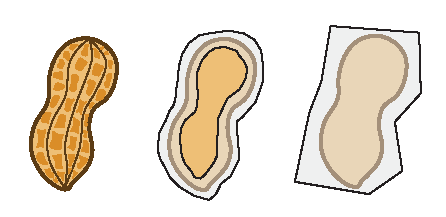
\includegraphics[width=0.9\linewidth]{figures/chap1/enclosing_geometry.pdf}
  \caption{包围几何中壳结构与笼结构的关系示意。}
  \label{fig:chap1_enclosing_geometry}
\end{figure}

\begin{figure}[htbp]
  \centering
  \includegraphics[width=0.9\linewidth]{figures/chap1/shell_app.pdf}
  \caption{壳结构在几何处理中的典型应用示意。}
  \label{fig:chap1_shell_app}
\end{figure}
与壳结构不同，笼结构通常仅由单层外边界表面构成，不显式包含与之配对的内表面。它以较为简化的边界网格包围目标对象，并将其内部视为一个整体控制域；目标几何嵌入其中，通过定义在笼边界上的控制变量及其向内部的传播机制响应外部操作。由于笼结构仅保留外表面，表示更紧凑、自由度更集中，因此更适合作为几何编辑与形变控制的操作界面。借助各类广义坐标或插值函数，笼边界上的位移、旋转和高阶控制量可以稳定传递到内部目标对象，从而支持交互式建模、角色动画和数字资产复用等任务。


\begin{figure}[htbp]
  \centering
  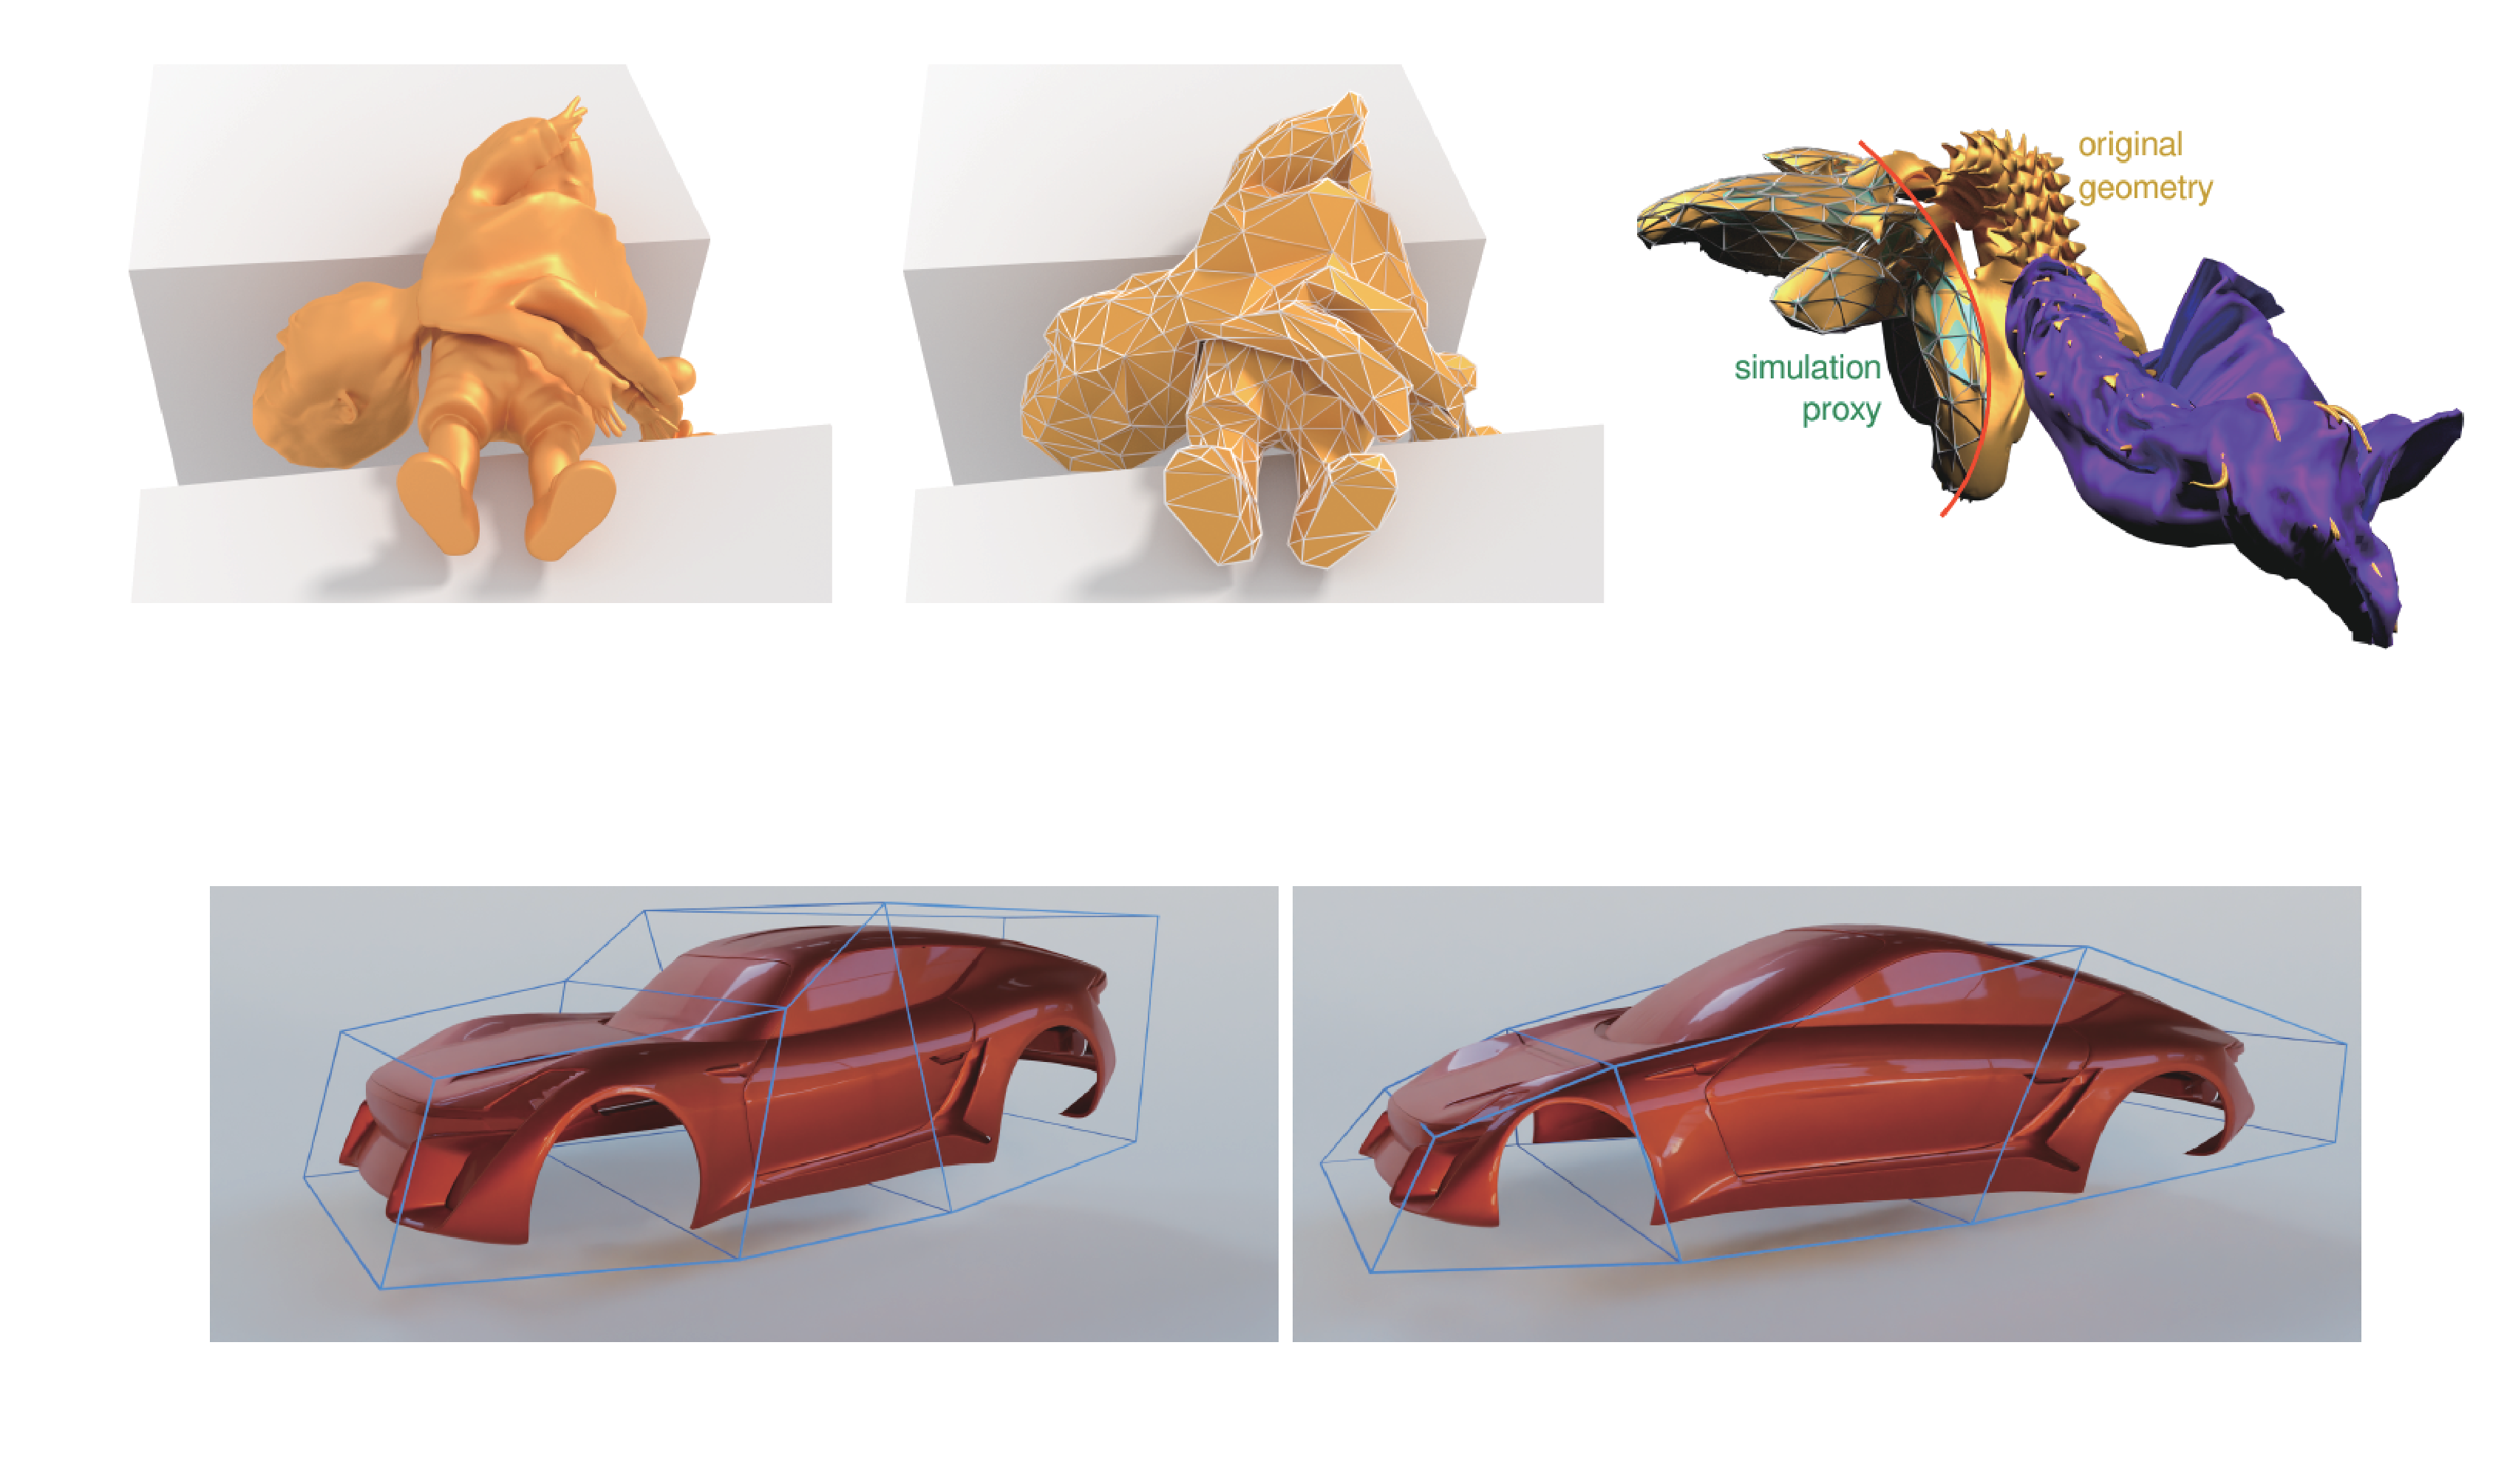
\includegraphics[width=0.9\linewidth]{figures/chap1/cage_app.pdf}
  \caption{笼结构在几何处理中的典型应用示意。}
  \label{fig:chap1_cage_app}
\end{figure}
壳结构与笼结构虽然同属包围几何，但面向的计算模式并不相同。壳结构依托内外两层边界界定的壳体区域，更适合承载投影、对应建立以及围绕壳体内部组织的映射计算；笼结构则依托单层外边界提供的控制界面，更适合通过边界约束向内部传播形变与属性。二者的共同点在于，它们都为复杂几何处理提供了一个比原始对象更规整、更可控的中间域。它们能否真正发挥作用，首先取决于该包围域能否被稳定识别，其次才取决于能否在该域及其内部构造出稳定、有效且质量足够高的几何映射。

对于规则且严格闭合的水密边界，已有多种包含查询方法可以完成内外判定，因此这一问题常被视为一个隐含前提。然而，实际应用中的包围几何并不总是水密，尤其在使用 CAD 软件生成或编辑的曲边形状中，边界常会出现缝隙、破碎或其他脏几何。此时，若仍依赖基于离散近似或局部线性化的判定策略，就很难同时兼顾几何精度、鲁棒性与查询效率。于是，鲁棒高效的包含查询不再只是附属操作，而成为采样、积分、区域组织、边界条件建立以及后续映射计算的基础环节。基于这一点，下一节进一步讨论本文主线上的包围几何内几何映射及其质量需求。
\section{包围几何内的映射}

在包围几何中，映射主要涉及两类问题：

\begin{figure}[htbp]
  \centering
  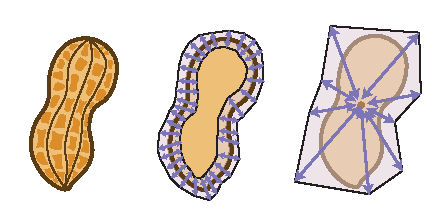
\includegraphics[width=0.9\linewidth]{figures/chap1/geometry_mapping.pdf}
  \caption{包围几何内壳空间映射与笼空间映射示意。}
  \label{fig:chap1_geometry_mapping}
\end{figure}

\begin{enumerate}
  \item \textbf{壳空间中的映射。} 以壳结构的边界曲面或壳体区域为定义域，直接构造向量值映射 $\mathbf{f}$。这类问题更关注壳体区域中的几何过渡、边界对应以及映射的双射性与光滑性。
  \item \textbf{笼空间中的映射。} 以笼结构围成的控制域为定义域，构造坐标函数 $\{w_i\}$ 并由其诱导映射。这类问题更关注边界控制量向内部的稳定传播，以及插值性、局部性与形变质量。
\end{enumerate}

为便于讨论，本文将这两类问题统一表述为如下函数构造问题：在域 $\Omega \subset \mathbb{R}^d$ 上构造向量值映射
\begin{equation}
  \mathbf{f}: \Omega \rightarrow \mathbb{R}^d,
\end{equation}
或构造一组标量坐标函数 $\{w_i:\Omega\rightarrow\mathbb{R}\}$，并通过这些坐标函数对边界控制量进行插值，从而得到相应映射。前者主要对应壳空间中的映射，后者主要对应笼空间中的映射。
在离散层面，$\Omega$ 可以由壳面的三角网格、壳体区域的体网格，或笼内部的采样点集表示，$\mathbf{f}$ 或 $\{w_i\}$ 则在相应的顶点或单元上离散。
\subsection*{映射质量与应用需求}

映射质量不仅是理论上的性质，也直接决定属性传递与几何编辑能否稳定进行。

\begin{itemize}
  \item \textbf{几何属性传递。}
  若能在源域与目标域之间构造稳定映射 $\mathbf{f}$，则颜色、纹理坐标、法向、位移、材料参数等属性即可通过推前或拉回（push-forward/pull-back）传递到目标模型。
  在这一过程中，映射的双射性与畸变水平直接影响结果是否出现重叠、撕裂或模糊。
  \item \textbf{几何编辑。}
  在笼编辑中，坐标函数 $\{w_i\}$ 的光滑性决定形变的连续性与视觉自然度；
  共形性、低扭曲与局部性则关系到细节保持和局部控制能力；
  若映射在编辑过程中发生折叠，还可能引发自交与不可逆形变，进而影响后续动画与仿真。
\end{itemize}

因此，本文关注的并非仅仅是“能否构造一个映射”，而是“能否构造一个\emph{可直接服务于下游任务}的高质量映射”。
\section{包围几何内的映射构造目标}

本文所讨论的“高质量映射”并非单一指标，而是一组与下游任务直接相关的性质。对包围几何内的映射而言，问题的关键不只是“是否存在一个映射”，而是能否在满足应用需求的前提下，同时兼顾几何质量、边界控制与数值可计算性。综合前述讨论，映射构造的核心目标可概括为：

\begin{enumerate}
  \item \textbf{双射性与可逆性：} 对壳空间中的映射，应在离散意义下尽量保证局部 Jacobian 不翻转（$\det J_{\mathbf{f}} > 0$），并在可能情况下获得全局单射，从而避免折叠与自交。
  \item \textbf{光滑性：} 相比仅有 $C^0$ 连续性的映射，具有 $C^1/C^2$ 连续性的映射能够显著减少折痕与尖峰伪影，对形变传播以及法向、曲率等高阶属性的稳定传递尤为重要。
  \item \textbf{共形性与低扭曲：} 根据任务需求，映射应尽量保持局部角度结构，并控制剪切、拉伸与扭曲，以避免局部形状在传递或形变过程中发生明显失真。
  \item \textbf{边界控制与约束一致性：} 映射或坐标应准确响应边界给定的控制条件。对笼坐标而言，这通常表现为严格的边界插值（控制点处 Kronecker Delta 性质）、线性精确性式~\ref{eq:barycentric} 以及稳定的局部控制能力。
  \item \textbf{效率与可复现：} 方法应能在常见网格规模下高效求解，最好具有可预分解或可重用的线性系统结构，并给出清晰的离散化与实现细节。
  \item \textbf{可验证性：} 方法应能对映射质量给出数值证据或证书，例如翻转检测、畸变上界估计以及条件数/稳定性分析，以降低隐藏失效的风险。
\end{enumerate}

上述目标在壳空间映射与笼空间映射中具有不同侧重，因此有必要分别分析。

\subsection{壳空间中的映射：双射性与光滑性}

壳空间中的映射可以看作一层层面之间的映射关系，例如外层与内层之间的对应，或沿壳体厚度方向的过渡映射。这类映射首先承担投影、包覆和边界传递的作用，因此其核心性质集中在双射性与光滑性上。

\begin{itemize}
  \item \textbf{双射性。} 若层与层之间的映射失去单射性，壳空间中便会出现折叠、自交或覆盖混乱，进而破坏投影关系和后续属性传递的正确性。因此，壳空间映射首先需要尽量保证局部不翻转，并在可能情况下保持全局可逆。
  \item \textbf{光滑性。} 壳空间映射不仅要建立对应关系，还要为后续的内部传播提供稳定边界条件。若映射不够光滑，局部几何误差会在传递过程中被放大，影响属性场、法向以及形变结果的连续性。
\end{itemize}

基于这一点，本文在壳结构上将问题聚焦为\textbf{光滑双射}映射的构造，并围绕可控的形变能量与可验证的无翻转机制展开研究。

然而，这一目标在离散壳结构上并不容易实现。壳空间映射既要在层间建立稳定的一一对应，又要避免局部翻转、自交与投影不连续；与此同时，为了服务属性传递和后续内部传播，映射还需要保持足够的光滑性。双射性与光滑性在实际构造中往往相互牵制，这使得壳结构上的高质量投影成为一个具有明显挑战性的问题。

\subsection{笼空间中的映射：共形性、扭曲控制与边界控制}

笼空间中的映射本质上是在笼所围成的体域内传播边界控制量，因此可以看作一种体积映射或体域中的坐标传播机制。与壳空间中的层间映射不同，这类映射需要把边界上的位移、旋转或其他控制信息稳定地传递到整个内部区域。其双射性通常主要通过笼边界的控制来保证；当笼边界在编辑过程中保持不自交时，诱导得到的内部映射通常也更容易保持可逆。在此基础上，笼空间映射仍需兼顾光滑性，并进一步关注共形性、扭曲性质以及边界控制性质。

\begin{itemize}
  \item \textbf{共形性。} 当映射尽量保持局部角度结构时，内部形变会更加自然，局部细节也更不容易因角度畸变而失真。这一点对编辑任务和属性传递都很重要。
  \item \textbf{扭曲控制。} 笼空间映射作用于体域内部，若剪切、拉伸或扭曲过大，就容易产生不自然的体积变形和局部伪影。因此，控制扭曲是保证形变质量的关键要求。
  \item \textbf{边界控制。} 笼方法的核心优势在于由边界控制内部，因此映射必须准确响应边界条件，保持严格插值、线性精确性以及可预期的局部控制能力，否则控制点的几何意义就会被削弱。
\end{itemize}

许多经典坐标都可以理解为某类 PDE 的边值解，例如调和坐标对应 Laplace 方程，双调和坐标对应 biharmonic 方程。本文围绕上述性质，在笼结构上沿两条路线展开：

\begin{itemize}
  \item \textbf{光滑性与共形性：柯西坐标。}
  面向需要角度保持的编辑与传递任务，本文构造一类具有共形倾向的坐标体系。其核心思想是利用与柯西--黎曼条件相关的结构，将“坐标场”与“共形结构”联系起来，从而在笼内部获得更平滑、角度畸变更小的映射。
  \item \textbf{光滑性、边界控制与低扭曲：双调和坐标。}
  面向自然形变与扭曲抑制需求，本文研究以双调和算子为基础的高阶坐标构造，并结合插值约束与畸变正则化，使形变在严格满足边界控制的同时，在内部呈现更自然的弯曲传播和更低的扭曲。
\end{itemize}

对于高阶柯西坐标而言，困难并不仅在于将线性笼推广到曲边笼，更在于推广后仍需同时保持闭式可解、导数可计算以及插值性、线性精确性与共形特性的协调统一。若缺乏统一的解析表达，曲边笼上的高质量编辑就很难兼顾精度、效率与可用性。

对于高阶双调和坐标而言，挑战则主要体现在边界控制与内部低扭曲之间的平衡。高阶曲边笼虽然提升了边界表达能力，但也使边值问题、离散求解与形变控制更为复杂。若希望在严格边界插值、内部自然传播和求解稳定性之间取得兼顾，就需要构造适用于高阶笼的新型双调和坐标框架。

由此可见，壳空间映射与笼空间映射虽然都服务于包围几何上的高质量映射，但它们关注的核心性质并不相同：前者重点在于双射性与光滑性，后者则在光滑性的基础上进一步强调共形性、扭曲控制与边界控制。下一节将在此基础上概括本文围绕这些目标展开的三项具体工作。
\section{本文内容与结构安排}

在上一节明确映射构造目标后，本节进一步概括本文的主要内容与整体结构。整体框架如图~\ref{fig:chap1_structure} 所示，本文围绕“包围几何上的高质量映射”展开，具体包含四项核心工作：

\begin{figure}[htbp]
  \centering
  
\includegraphics[width=0.92\linewidth]{chap1_structure.png}
  \caption{文章结构。}
  \label{fig:chap1_structure}
\end{figure}

\begin{enumerate}
  \item \textbf{高效鲁棒的包围几何的内外判断。}
  本文研究由有理参数曲线构成的二维包围边界上的鲁棒包含查询问题。方法上，本文以广义环绕数作为统一判据，将有理参数曲线上的内外判断转化为多项式 B\'{e}zier 曲线上的有理多项式积分，并借助留数定理给出闭式计算表达；同时进一步处理查询点位于边界上的特殊情形，并推导广义环绕数导数。由此得到的方法可在复杂曲边边界下实现高效、稳定的内外判定，并为曲线方向分析与相关几何处理任务提供统一的计算基础。
  \item \textbf{壳结构上的光滑双射投影。}
  本文研究壳空间内的光滑双射投影问题，提出一种高阶壳表示及其实用构造算法。该方法以初始线性壳为起点，通过边塌缩、几何优化、边翻转与棱柱缩放等局部操作，在满足包围约束、角度约束和厚度约束的前提下，逐步得到由高阶三角棱柱组成的壳结构，并在壳内构造连续向量场以定义投影算子。实验表明，该方法能够稳定生成高阶壳，并获得更光滑、更均匀的壳空间投影，适合支撑重网格化后的属性回传、布尔运算与位移贴图等应用。
  \item \textbf{笼结构内的高阶柯西坐标。}
  本文研究高阶笼上的 Cauchy 坐标，给出坐标、导数与相关有理积分的统一闭式解析表达。针对传统线性输入笼对复杂边界贴合不足、边界附近光滑性欠佳的问题，本文将 Cauchy 坐标推广到高阶输入笼，并基于留数定理构建有理积分的闭式求解流程。实验结果表明，高阶笼能够在保持保角变形优势的同时提供更贴合边界、更平滑且更符合编辑意图的结果。
  \item \textbf{笼空间中的半解析半数值的高阶双调和坐标。}
  本文研究高阶笼上的双调和坐标，提出面向曲边边界的高阶 BEM 求解框架。该方法通过高阶边界单元、高阶形函数与统一代数系统，将双调和边值问题推广到高阶笼，并结合不同边界导数设计与加权策略，在严格边界插值与内部低扭曲之间提供连续可调的平衡机制。实验结果表明，本文方法能够在复杂曲边笼编辑中提供更稳定的内部形变传播，并在变形自然性与边界可控性之间取得更灵活的折中。
\end{enumerate}

在上述四项工作的支撑下，本文进一步讨论它们在\textbf{几何属性传递}、\textbf{几何编辑}与\textbf{曲线查询}中的应用：前两类任务依赖高质量映射与坐标构造，后一类任务则依赖曲边边界上的鲁棒内外判定。

除本章外，全文其余章节安排如下：

\begin{itemize}
  \item 第2章介绍相关理论基础与研究现状，主要包括几何映射的离散表示、畸变度量、广义重心坐标以及基于 PDE 的坐标构造等内容。
  \item 第3章围绕高效鲁棒的包围几何的内外判断展开，以有理参数曲线构成的二维包围边界为对象，讨论广义环绕数的闭式计算、边界点情形、导数计算及其在曲线查询中的效率表现。
  \item 第4章研究壳结构上的光滑双射投影模型、算法与性质，并通过属性传递实验验证方法的有效性。
  \item 第5章介绍高阶柯西坐标的构造方法，讨论其数学性质、离散实现以及在笼编辑中的表现。
  \item 第6章从第5章的共形坐标出发，转向研究边界可控且内部低扭曲的高阶双调和坐标，重点讨论其半解析半数值构造、变形控制以及与经典坐标的对比实验。
  \item 第7章总结全文工作，并讨论后续可进一步开展的研究方向。
\end{itemize}






